\newpage
\begin{center}
 \textbf{Segunda Opción (Mercado bursátil)}
\end{center}

a) Para 90 días antes del vencimiento:

%La tabla ira centrada
\begin{center}
 \renewcommand{\arraystretch}{1.5}% Margenes de las celdas
 %Creación de la cuadricula de 3 columnas
 \begin{longtable}[H]{|p{0.5\linewidth}|p{0.5\linewidth}|}
  %Creamos una linea horizontal
  \hline
  %Definimos el color de la primera fila
  \rowcolor[HTML]{FFB183}
  %%%%% INICIO ASIGNACIÓN FECHA FOCAL %%%%%%%
  %%%%%%%%%% INICIO TITULO
  %Lo que se hace aquí es mezclar las 3 columnas en una sola
  \multicolumn{2}{|c|}{\cellcolor[HTML]{FFB183}\textbf{1. Asignación período focal}}                   \\ \hline
  %%%%%%%%%% FIN TITULO
  %%%%% INICIO DECLARACIÓN DE VARIABLES %%%%%%%
  \multicolumn{2}{|c|}{$pf = 90 \textit{ pdv}$}                                                      \\ \hline
  %%%%%%%%%% INICIO TITULO
  %Lo que se hace aquí es mezclar las 3 columnas en una sola
  \multicolumn{2}{|c|}{\cellcolor[HTML]{FFB183}\textbf{2. Declaración de variables}}                 \\ \hline
  %%%%%%%%%% FIN TITULO
  %%%%%%%%%% INICIO DE MATEMÁTICAS
  %Cada & hace referencia al paso de la siguiente columna
  $F =  100 \ COP$                   & $P_r = ? \ COP$                                                            \\
  $n  = \frac{90}{365} = 0.247\% \ pdv$     & $P_v=?\ COP$                                                             \\
  $i_r = 30\%\textit{ pdv}  $  & $i_v=?\% $                                                             \\
  $com_v = 0,5\%\textit{ pdv}$ &    $i_{r}+comv = P_{v}$                                                                 \\ \hline
  %%%%%%%%%% FIN DE MATEMÁTICAS
  %%%%% FIN DECLARACIÓN DE VARIABLES


  %%%%% INICIO FLUJO DE CAJA
  \rowcolor[HTML]{FFB183}
  \multicolumn{2}{|c|}{\cellcolor[HTML]{FFB183}\textbf{3. Diagrama de flujo de caja}}                \\ \hline
  \multicolumn{2}{|c|}{ 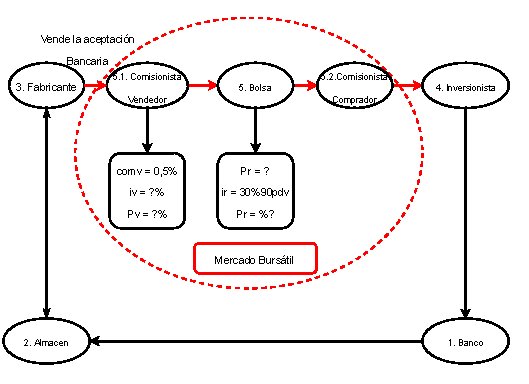
\includegraphics[trim=-78 -5 -78 -5]{3_Capitulo/img/ejemplos/7/Capitulo3Ejercicio7a3.pdf} }  \\ \hline
  %%%%%% FIN FLUJO DE CAJA

%%%%% INICIO DECLARACIÓN FORMULAS
  \rowcolor[HTML]{FFB183}
  \multicolumn{2}{|c|}{\cellcolor[HTML]{FFB183}\textbf{4. Declaración de formulas}}                  \\ \hline
  \multicolumn{2}{|C{\textwidth}|}{
  $F = P(1 + i)^n $ \hspace{2mm} Valor futuro 
  
  $I_r$ para calcular $p_r$    

  $i_r$ comv para calcular $p_c$

  $V_v=?$
  }
  \\ \hline
  %%%%% FIn  DECLARACIÓN FORMULAS
  \rowcolor[HTML]{FFB183}
  \multicolumn{2}{|c|}{\cellcolor[HTML]{FFB183}\textbf{5. Desarrollo matemático}}                    \\ \hline
  %Mezclamos 3 columnas y pondremos el dibujo
  %%%%%%%%%%%%% INSERCIÓN DE LA IMAGEN
  %Deberán descargar las imágenes respectivas del drive y pegarlas en la carpeta
  %n_capitulo/img/ejemplos/1/capitulo1ejemplo1.pdf  (el /1/ es el numero del ejemplo)
  \multicolumn{2}{|C{\linewidth}|}{

  $P_r =   100 \ COP (1 + 0,30)^\frac{-90}{365} = 93,7356\% \equiv 4{.}686{.}780 \ COP$

  $i_v = 0,5\% \hspace{1mm} pdv + 30\%\hspace{1mm}pdv = 30,5\% \hspace{1mm}pdv$

  $Pv =  100\ COP(1 + 0, 3050)^\frac{-90}{365}= 93,6469\% \equiv  4{.}682{.}345\ COP $

  }                                                                                                  \\ \hline

  %%%%% INICIO DECLARACIÓN FORMULAS
  %%%%%%%%%%% INICIO TITULO
  \rowcolor[HTML]{FFB183}

  %%%%%% INICIO RESPUESTA
  \rowcolor[HTML]{FFB183}
  %%%%%%%%%%INICIO TITULO
  \multicolumn{2}{|c|}{\cellcolor[HTML]{FFB183}\textbf{6. Respuesta}}                                \\ \hline
  %%%%%%%%%% FIN TITULO
  %%%%%%%%%% INICIO RESPUESTA MATEMÁTICA
  \multicolumn{2}{|C{\textwidth}|}{
  $Pr =   4{.}686{.}780 \ COP$

  $iv = 30, 5\% \hspace{1mm} pdv$

  $Pv =   4{.}682{.}345 \ COP$

  $P_v = 93,6469\% < p_r = 93,7356?\%$
  }                                                                                                  \\ \hline
  %%%%%%%%%% FIN MATEMÁTICAS

  
  %%%%%% FIN RESPUESTA
 \end{longtable}
 %Se crean dos lineas en blanco para que no quede el siguiente texto tan pegado
 %\newline \newline %USARLO SI CREES QUE ES NECESARIO
\end{center}
